\section{Future improvements}

As shown in this chapter, despite the use of MVA techniques, the kinematic reconstruction of the $t\bar{t}H$ system remains challenging due to the high combinatorial background. With higher luminosities since only a small fraction of $t\bar{t}H$ events have the top and Higgs bosons with sufficiently high momentum, the boosted regime can improve significantly the signal-to-background ratio and give the possibility to reconstruct the Higgs-boson candidate. In the boosted regime, the two $b$-quarks from the Higgs-boson decay will have small angular separation and would be reconstructed as a single jet (see figure \ref{sec:ttH:fig:boost}), whose mass would peak at the correct Higgs-boson mass.

\begin{figure}[h!]
\centering
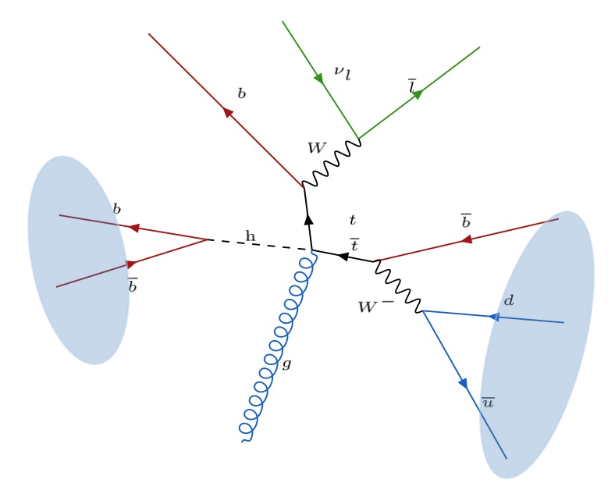
\includegraphics[width=0.5\textwidth]{figures/ttH/boosted.png}
\captionsetup{width=0.85\textwidth} \caption{\small Sketch of boosted $t\bar{t}H$ event in which the Higgs and the hadronic top are reconstructed as large-$R$ jets. From reference \cite{Moretti:2015vaa}.}
\label{sec:ttH:fig:boost}
\end{figure}


In recent publications \cite{Moretti:2015vaa} it is highlighted that the application of these techniques to the $t\bar{t}H$ search will represent a major improvement in sensitivity, allowing the observation of the Higgs boson in this production mode, as well as the most precise measurement of the top-Higgs Yukawa coupling.
The boosted scenario can help as well in measuring the Higgs-boson \pt distribution in $t\bar{t}H$ production, which is one of the main probes for a CP-odd component in the top-Higgs interaction \cite{Degrande:2012gr}. Boosted techniques in the associated $t\bar{t}$ production mode can be exploited as well to perform searches of light scalars (<100 \gev) decaying to $b\bar{b}$ at the LHC (see appendix \ref{App:AppendixA}).\par
In the context of the inclusive search, the use of jet-flavour information by exploiting the shape of the MV2c10 variable (referred to as "continuous $b$-tagging"), as well as adding kinematic information via sophisticated techniques such as the matrix-element method, will further improve the discriminating power of the classification BDT.
Finally, as already discussed in section \ref{chp:VLQ:sec:improvemente}, a reduced modelling uncertainties of the $\ttbar$+jets background through higher-order calculations (MEPS@NLO) and validated with data measurements will allow a reduction in the systematic uncertainties for the main background, further boosting the sensitivity of this search.

